\chapter{Beleuchtung (Fortsetzung)}
\section{Flatshading}
Alle Knoten einer Fläche habe die gleiche Normale\\
Normale ermitteln + normieren (u.U. Gewichten z.B. Fläche oder Winkel)
\begin{figure}[H]
	\centering
	\begin{subfigure}{0.45\textwidth}
	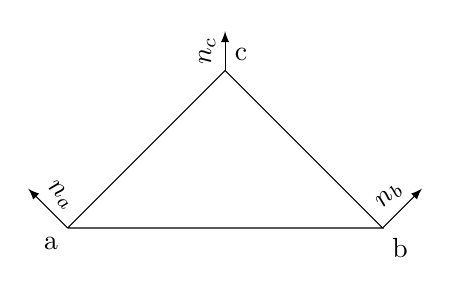
\begin{tikzpicture}[scale=2]
	\draw (-1,0) node[anchor=north east] {a}--(1,0) node[anchor=north west] {b}--(0,1) node[anchor=south west] {c}--(-1,0);
	\draw[-latex] (-1,0)--(-1.25,.25) node[above, pos=.5, sloped] {$n_a$};
	\draw[-latex] (1,0)--(1.25,.25) node[above, pos=.5, sloped] {$n_b$};
	\draw[-latex] (0,1)--(0,1.25) node[above, pos=.5, sloped] {$n_c$};
	\end{tikzpicture}
\end{subfigure}
\begin{subfigure}{0.45\textwidth}
	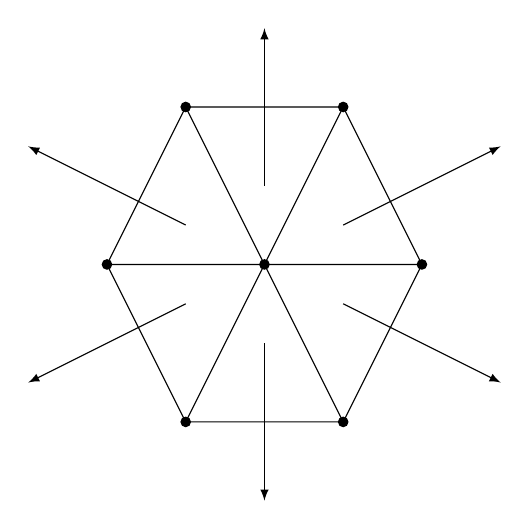
\begin{tikzpicture}[scale=2]
	\draw (-1,0)--(-.5,1)--(.5,1)--(1,0)--(.5,-1)--(-.5,-1)--(-1,0)
	(-1,0)--(0,0)
	(-.5,1)--(0,0)
	(.5,1)--(0,0)
	(1,0)--(0,0)
	(.5,-1)--(0,0)
	(-.5,-1)--(0,0);
	\filldraw
	(-1,0)circle (0.03)
	(-.5,1)circle (0.03)
	(.5,1)circle (0.03)
	(1,0)circle (0.03)
	(.5,-1)circle (0.03)
	(-.5,-1)circle (0.03)
	(0,0)circle (0.03);
	\draw[-latex] (0,.5)--(0,1.5);
	\draw[-latex] (-.5,.25)--(-1.5,.75);
	\draw[-latex] (-.5,-.25)--(-1.5,-.75);
	\draw[-latex] (0,-.5)--(0,-1.5);
	\draw[-latex] (.5,.25)--(1.5,.75);
	\draw[-latex] (.5,-.25)--(1.5,-.75);
%	\draw[-latex] (-1,0)--(-1.25,.25) node[above, pos=.5, sloped] {$n_a$};
%	\draw[-latex] (1,0)--(1.25,.25) node[above, pos=.5, sloped] {$n_b$};
%	\draw[-latex] (0,1)--(0,1.25) node[above, pos=.5, sloped] {$n_c$};
	\end{tikzpicture}
	
	\end{subfigure}
\end{figure}
\pagebreak
\subsubsection{Lambert}
\[ \text{I}_D = \text{I}_L \cdot \left( n^T \cdot \ell \right) \]
\begin{figure}[H]
	\centering
	\begin{tikzpicture}
	\draw (-1,0)--(1,0);
	\node at (0,1) (a) {};
	\node at (-.707,.707) (c) {};
	\draw[-latex] (0,0) node (b){}--(0,1) node[above] {$n$};
	\draw[-latex] (0,0)--(-0.707,0.707) node[above] {$\ell$};
	\draw pic[draw, "$\varphi$" , angle eccentricity=1.2, angle radius=15] {angle=a--b--c};
	\draw[dashed] (-0.707,0.707)--(-2*0.707,2*0.707) node [scale=0.05,solid, draw,star,star points=12,star point ratio=28] {};  %node[scale = 1.5] {\textasteriskcentered};
	\end{tikzpicture}
\end{figure}

\begin{align*}
	x' = M\cdot x && E = & \{ x | n^T x = n_0 \} && M\in \mathbb{R}^{3\times 3}\\
	              &&     & \{ Mx | n^T x = n_0 \} && \\
	\text{z.B. } M = R && & R^{-1} = R^T && R: \text{ Rotation}
\end{align*}
\begin{align*}
	&\text{Transformationsregel }&x' &=\mathbb{R}x &&\\
	&&n' &=\mathbb{R}n &&  
\end{align*}
\paragraph{Behauptung}
\begin{align*}
	x'&=Mx	&\text{für Rotationen} & \left( R^{-1} \right)^T = \mathbb{R}\\
	n'&=\left( M^{-1} \right)^Tn   &&
\end{align*}
\paragraph{Beweis}
\begin{align*}
	&& n'^Tx' = \left( \left( M^{-1} \right)^T n \right)^T Mx &= n^T M^{-1^{T^T}}\cdot Mx = n^TM^{-1}Mx\\
	&&&=n^Tx = n_0
\end{align*}
\paragraph{Qt}
$\left( M^{-1} \right)^T$. \texttt{QMatrix4x4::normalMatrix}


\chapter{Einschub: virtual Trackball}
\begin{figure}[H]
	\centering
	\begin{tikzpicture}[scale = 2]
		\draw[-latex] (-1.4,0) -- (1.4,0);
		\draw[-latex] (0,-1.4) -- (0,1.4);
		\draw (0,0) circle (1);
		\node[inner sep = 0, outer sep = 0, label = $a$] at (-.5, .5) (a) {};
		\node[inner sep = 0, outer sep = 0, label = $b$] at (.5,.2) (b) {};
		\draw (0,0) -- (a) -- (b) -- (0,0);
		\node at (-.5, .5, {sqrt(1-.5)}) (a') {};
		\node at ( .5, .2, {sqrt(1-.25-0.04)}) (b') {};
		\pgfmathsetmacro{\xx}{0.5*sqrt(0.71)-sqrt(0.5)*0.2}
		\pgfmathsetmacro{\y}{sqrt(0.5)*0.5+0.5*sqrt(0.71)}
		\pgfmathsetmacro{\z}{-0.5*0.2 - 0.25}
		\pgfmathsetmacro{\len}{1 / sqrt( \xx*\xx + \y*\y + \z*\z )}
		\edef\l{\len}
		\node[inner sep = 0] at (\len*\xx,\len*\y,\len*\z) (x) {};
		\draw[-latex] (0,0,0) -- (x) node[above] {$r$};
		\draw[{Latex[length=6]}-, line width = 1] (-.5, .5)--++(-.075,-.15) node{};
		\draw[{Latex[length=6]}-, line width = 1] (.5,.2)--++(-.075,-.15) node{};
	\end{tikzpicture}
	\caption{Virtueller Trackball}
\end{figure}
\begin{align*}
	&& a & = \left( x_a, y_a, \sqrt{1 - x_a^2 - y_a^2} \right) &&\\
	&& b & = \left( x_b, y_b, \sqrt{1 - x_b^2 - y_b^2} \right) &&\\
	&& r & = a\times b \pm \text{normieren}
\end{align*}
Bewege $a$ nach $b$ auf einem Großkreis\\
Normale der Großkreisebene ist $\frac{a\times b}{\left| a\times b \right|} = r \hat{=}$ Rotationsachse
\paragraph{Winkel}
\[ \cos\varangle(a,b) = \frac{a\cdot b}{\left| a\cdot b \right|} \]
\section{Formel von Rodriques}
\begin{align*}
	&& \text{Achse, Winkel} & \rightarrow \text{Rotationsmatrix} &&\\
	&& (r, \varphi) & \rightarrow R &|r| = 1&
\end{align*}
\begin{lstlisting}
QMatrix4x4 R;
R.rotate($\underset{\deg}{\underbrace{f}}, r$);
\end{lstlisting}
\begin{figure}[H]
	\centering
	\begin{subfigure}{.23\textwidth}
		\centering
		\begin{tikzpicture}[scale=2]
			\draw[-latex] (0,0,0) -- (1,0,0) node[below] {x};
			\draw[-latex] (0,0,0) -- (0,1,0) node[right] {y};
			\draw[-latex] (0,0,0) -- (0,0,1.5) node[below] {z};
			\draw[-latex, very thin, gray] (0,0,0) -- (0,0,-2);
			\draw (.5,.5,0) circle (.25);
			\coordinate (a) at (.5,.5,0);
			\coordinate (p) at ($ (.5,.5,0) + (0,0,0)!.45!90:(0,0,1) $);
			\coordinate (e) at (.5,.75,0);
			\draw[-latex] (.5,.5,0) -- (p) node[right, anchor = north west] {$p$};
			\draw (a) --++(0,0,.1)--++($(0,0,0)!.1!90:(0,0,1)$)--++(0,0,-.1) -- cycle;
			\node[inner sep = .1pt, circle, fill=black] at (.5, .465, 0) {};
			\draw[-latex] (a) -- (e) node[left, pos=.5] {$r$};
			\node[above] at (e) {$p'$};
			\pic[draw=black, angle eccentricity=1.2,angle radius=7] {angle=p--a--e};
			%\draw[very thin, gray] (a) --++(.3,0,0);
		\end{tikzpicture}
		\caption{$c=\left( r^Tp \right)r$}
	\end{subfigure}
	\begin{subfigure}{.23\textwidth}
		\centering
		\begin{tikzpicture}[scale=4]
		\draw (.5,.5,0) circle (.25);
		\coordinate (a) at (.5,.5,0);
		\coordinate (p) at ($ (.5,.5,0) + (0,0,0)!.45!90:(0,0,1) $);
		\coordinate (e) at (.5,.75,0);
		\draw[-latex] (.5,.5,0) -- (p) node[right, anchor = north west] {$p$};
		\draw[-latex] (a) -- (e) node[left, pos=.5] {$r$};
		\node[above] at (e) {$p'$};
		\pic[draw=black, angle eccentricity=1.2,angle radius=14] {angle=p--a--e};
		\coordinate (phi) at ($(a)+(20:.07)$);
		\node at (phi) {$\varphi$};
		\node[left] at (a) {$c$};
		%\draw[very thin, gray] (a) --++(.3,0,0);
		\end{tikzpicture}
		\caption{}
	\end{subfigure}
	\begin{subfigure}{.23\textwidth}
		\centering
		\begin{tikzpicture}[scale=2]
			\node[inner sep = 0, outer sep = 0] at (1,1) (c) {};
			\node[above] at (c) {c};
			\draw[-latex] (0,0)--(1,1) node[above, pos=.5] {$r$};
			\draw[-latex] (0,0)--($ (1,1) + (0,0)!.75!-90:(1,1) $) node[inner sep = 0, outer sep = 0] (p) {};
			\draw (p)--(1,1);
			\node[inner sep = 0, outer sep = 0] at (0,0) (0) {};
			\node[left] at (0) {$0$};
			\node[right] at (p) {$p$};
			\pic[draw=black, angle eccentricity=1.2,angle radius=20] {angle=p--0--c};
			\pic[draw=black, angle eccentricity=1.2,angle radius=10] {angle=0--c--p};
			\node[fill = black, inner sep = .25pt, circle] at ($(c) + (-90:.1)$) {};
			\node at ($(0) + (25:.25)$) {$\alpha$};
			\draw [decorate,decoration={brace,amplitude=20}] (0) -- (c) node [sloped, pos=.5, above, yshift=20] {$k^\ell$}; % Keine Ahnung mehr, was hier stand
		\end{tikzpicture}
		\caption{$\ell=r^Tp$}
	\end{subfigure}
	\begin{subfigure}{.23\textwidth}
		\centering
		\begin{tikzpicture}[scale=1.5]
		\draw (0,0) circle (1);
		\node at (1,0) (p) {};
		\draw[-latex] (0,0) -- (1,0) node[below, pos=.5] {$u$};
		\draw[-latex] (0,0) -- (0,1) node[left, pos=.5] {$v$};
		\draw[-latex] (0,0) -- ({cos(45)}, {sin(45)}) node (p') {};
		\node at (0,0) (0) {};
		\node[below] at (0) {$c$};
		\node[right] at (p) {$p$};
		\node[above right] at (p') {$p'$};
		\pic[draw=black, angle eccentricity=1.2,angle radius=20] {angle=p--0--p'};
		\node at (45/2:.3) {$\varphi$};
		\end{tikzpicture}
		\caption{$u = p - c $ \\ $v = r \times u$}
	\end{subfigure}
\end{figure}
\paragraph{zu c}
\begin{align*}
	&&\ell &= \cos \alpha \cdot |p|&&\\
	&&&= \frac{r^Tp}{\underset{=1}{\underbrace{\stkout{|r|}}}\stkout{|p|}}\stkout{|p|} 
\end{align*}

\begin{align*}
	Rp & = p' = c + \cos \varphi u + \sin \varphi v\\
	& = c + \cos \vektor{1\\0} + \sin \varphi \vektor{0\\1}\\
	& = c + \cos \varphi (p-c) + \sin \varphi \left( r \times (p-c) \right)\\
	& = (1 - \cos \varphi) c + \cos \varphi p + \sin \varphi (r\times p) & \text{da } r\times c & = 0\\
	& = (1 - \cos \varphi) \left( rr^t \right)p + \cos \varphi p + \sin \varphi \left( r^xp \right)&(AB)C &=A(BC)\\
	\Aboxed{&=(1-\cos\varphi) rr^T + \cos \varphi I + \sin\varphi r^x } & r^Tr & = \vektor{r_1^2&r_1r_2&r_1r_3\\r_2r_1&r_2^2&r_2r_3\\r_3r_1&r_3r_2&r_3^2}
\end{align*}
\subsection{dyadisches Produkt}
\begin{align*}
\left( rr^T \right)^T &= r^{T^T}r^T = rr^T&&\Rightarrow \text{symmetrisch}
\end{align*}